%=========================Preamble====================================%
\documentclass[12pt] {article}

\usepackage{graphicx}
\usepackage{subfig}
\usepackage[usenames]{color}
\usepackage[]{todonotes}
\usepackage{blindtext}
\usepackage{listings}
\usepackage{hyperref}

\newcommand{\ahmed}[1]{\todo[inline,color=blue!30]{\textbf{ahmed:} #1}}%set command to comment
\definecolor{figblue}{rgb}{0,0,1}%set color

\newcommand{\mohamed}[1]{\todo[inline,color=green!30]{\textbf{mohamed:} #1}}%set command to comment
\definecolor{figgreen}{rgb}{0,0.6,0}%set color

\newcommand{\final}{1}%Set to 1 to remove comments 

\ifthenelse{\equal{\final}{1}}%make sure comments don't show when \final = 1
{
\renewcommand{\mohamed}[1]{}
\renewcommand{\ahmed}[1]{}
}

\newcommand{\wes}{{\fontfamily{qcr}\selectfont wesBench}}
%=========================Doc====================================%
\begin{document}
\title{Characterization and Reverse-engineering Assignment - EEC 277}
\author{Ahmed H. Mahmoud and Mohamed El-Banna}
\date{7 February 2017} 
\maketitle


%=========================Intro====================================%
\section{Introduction}
This report is divided into two parts; performance analysis of the graphics card and reverse engineering to charactrize undocumneted features of the GPU. In the first part, we are going to characterize the performance of the two GPU using \protect{\wes} benchmark. The target here is to find the crossover point between the geometry/vertex stage and fragment/rasterization stage for different scenarios. Broadly speaking, the graphics pipeline overall performance is a function of the slowest of these two stages. It is well known that the geometry stage favors large primitive triangles since the speed of this stage is dependent on the operations-per-vertex. In contrast, rasterization stage favors small primitive triangles since a large triangle would require more fill operations \cite{Bethel_2010}.

Second part is concerned with detecting the precision of the graphic card. We first characterize the error associated with primitives math operations OpenGL. Additioanlly, we use a simple shader program to ensure the compliance of our GPU with IEEE-754 standards and to detect the rounding algorithm implemented. 

All the experiments presented in the report are done on NVIDIA GeForce GT 610 GPU on a Windows 7 machine with four-core Intel(R) Xeon(R) CPU of 3.7GHz and 32.0GB RAM. 



\newpage

\section{Part A}
%=========================Default Triangles====================================%
\subsection{Geometry Rate Vs. Fill Rate:}
The objective of first experiment is to find the crossover point for the unlit, untexture triangles between the fill rate and geometry rate in terms of triangle area in pixels.  This is done by testing both rates for different triangle sizes. The results are shown in Figure \ref{fig:fill_geo1}(a) on a log-log scale, where the fill rate (MFrags/Sec) increases as expected for small triangles and geometry rate (MVerts/Sec) decreases. The crossover point is between triangle area between $2^{10}$ and $2^{11}$ pixels. We notice that for triangle of size between $2^{1}$ to $2^{4}$ pixels the geometry rate is almost constant.  Even though the geometry rate is the highest but this could be due to more efficient use of caching. Since the triangles are of small size, and due to spatial locality, more triangle can be fetched and put into the cache. 

On the other side, the rapid change on the fill rate starts to slow down at triangle size greater than $2^{4}$ pixels. This is noticable since the fill rate curve can be approximated by a quadratic function for upto triangle size of $2^{4}$. After that, the curve takes a linear trend which is slower than quadratic trend. This could be due to the fact that the geometry stage is not sending enough work to the rasterization stage. So even the overall fill rate increases as the triangle size increases, but the slope of the curve is not the same overall.

\begin{figure}[!tbh]
 \centering  
 \subfloat[Default]
    {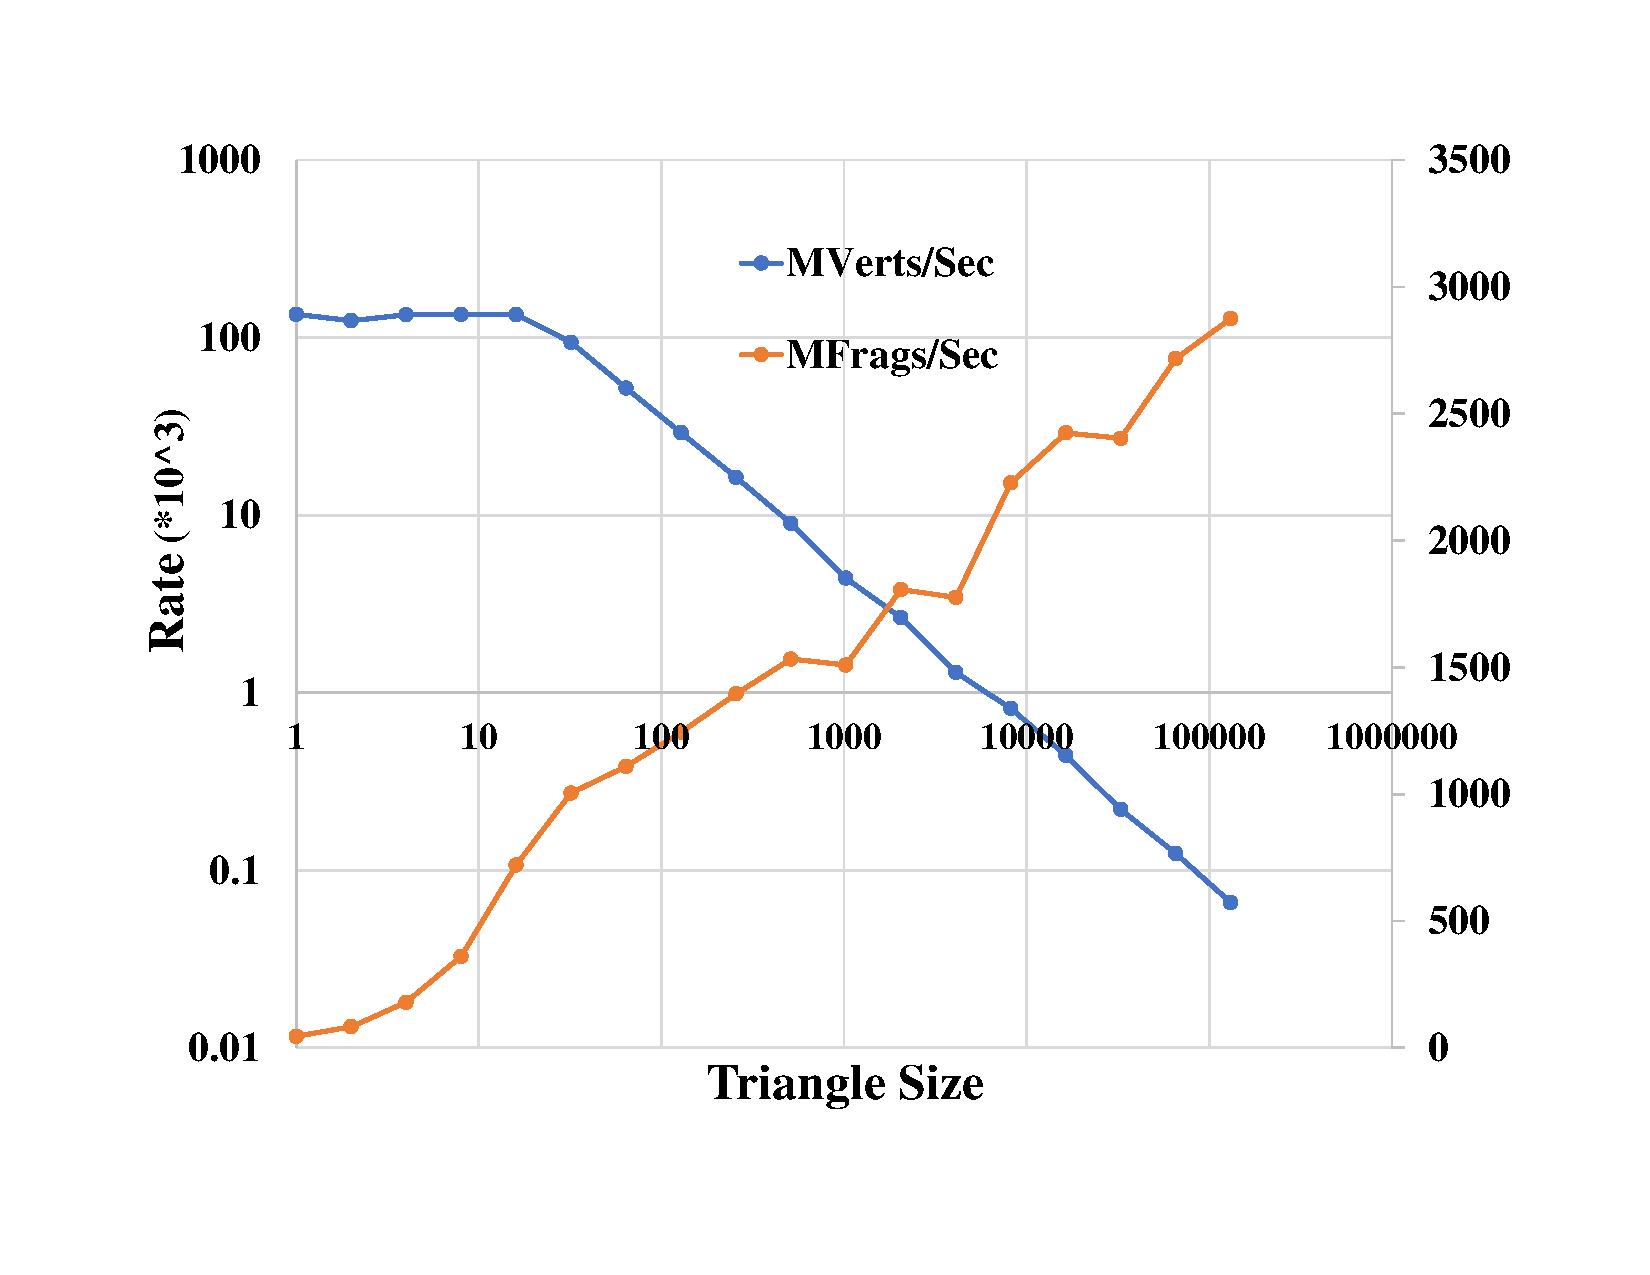
\includegraphics[width=0.49\linewidth]{fig/fill_geo.pdf}}   
 \subfloat[Lit Triangles]
   {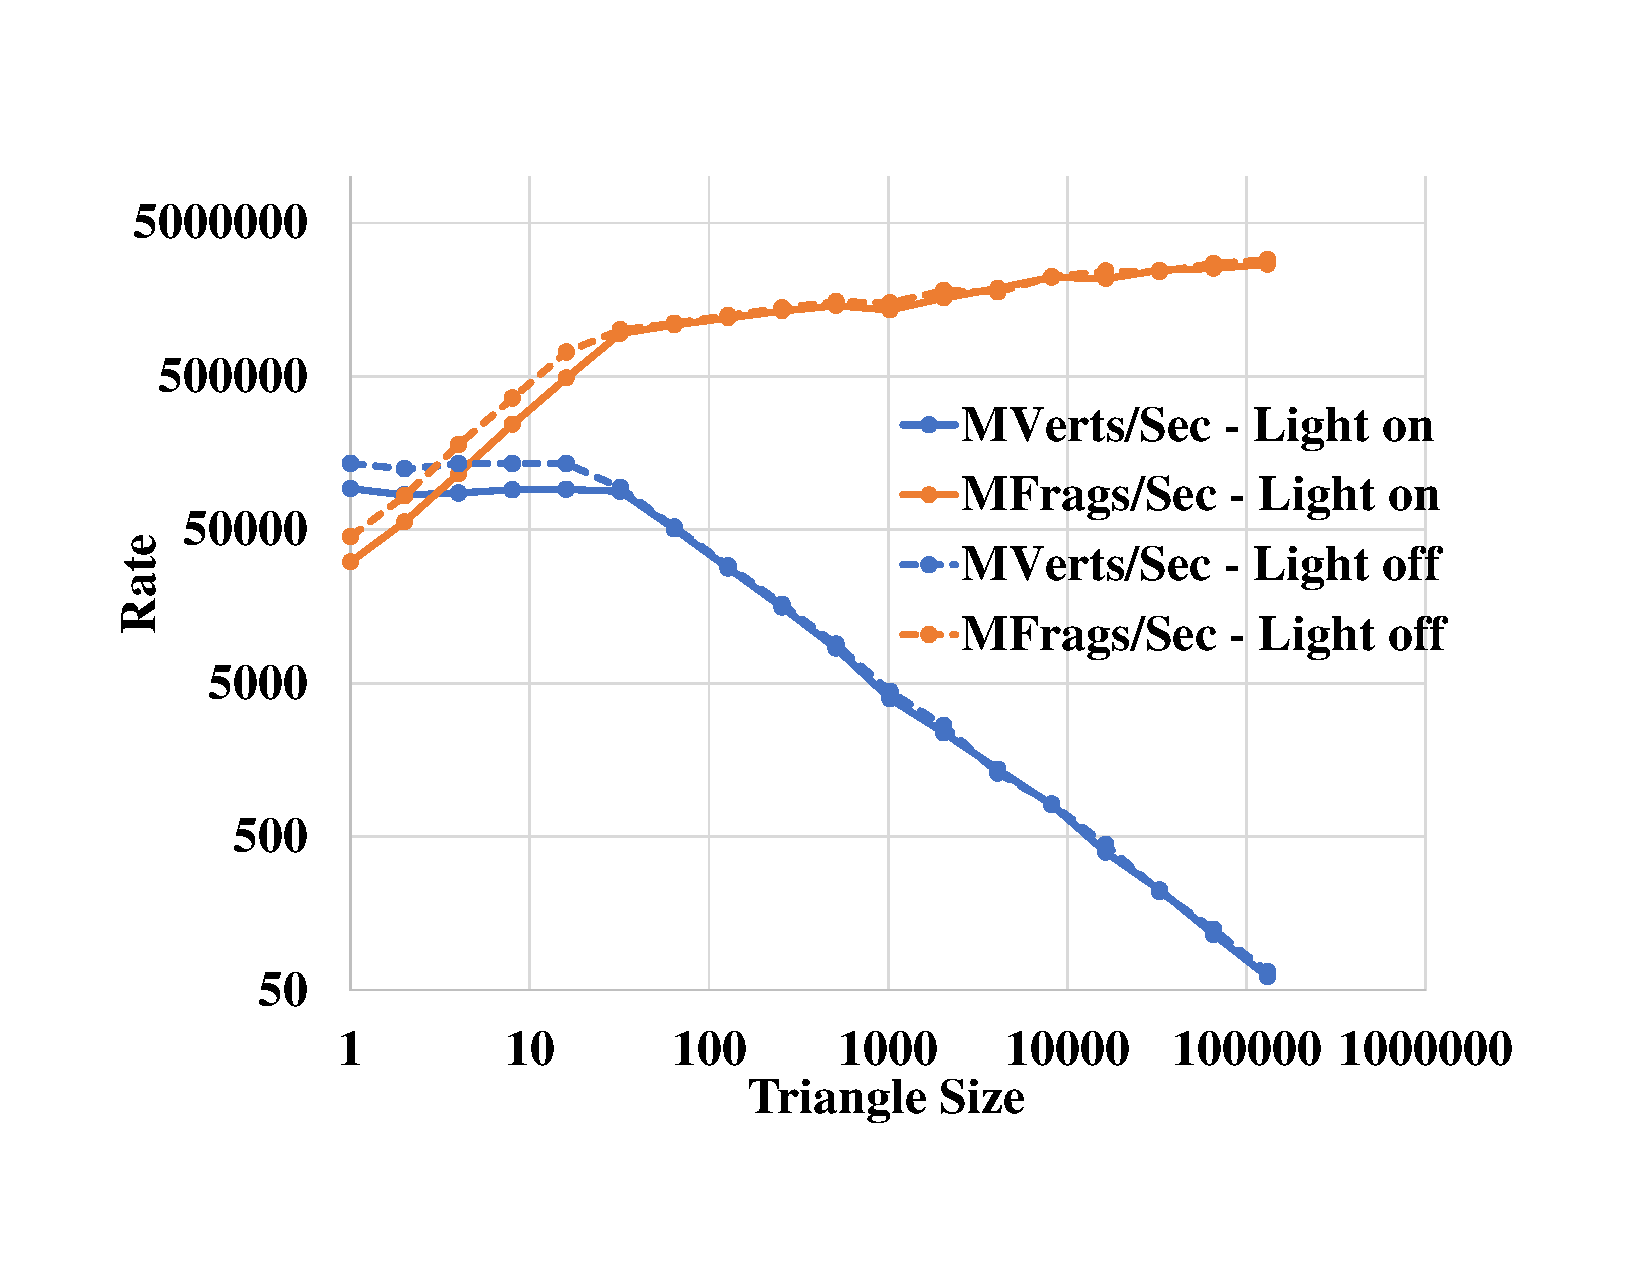
\includegraphics[width=0.49\linewidth]{fig/fill_geo_lit.pdf}}
  \caption{Performance and crossover point of the default settings in \protect{\wes} (a) and the lit triangles Vs. the default (unlit) triangles (b) in millions of vertices per second and millions of fragments per second.}
   \label{fig:fill_geo1}
\end{figure} 

%========================= Lit Triangles ====================================%
\subsection{Geometry Rate Vs. Fill Rate on Lit Triangles:}\label{sec:lit}
The previous test was done on unlit, untexture triangles which is the default setting in \protect{\wes}. Now we turn on the light on the triangles and do the same test and compare the results with the unlit triangles. The results are shown in Figure \ref{fig:fill_geo1}(b) where the crossover point is almost the same (we only notice it moved a little closer to triangle of size $2^{11}$). Additionally, we notice that the upper portion of the graph (towards triangle of size greater than $2^{5}$ pixels) of the geometry rate curve is identical i.e., the dotted and the solid lines overlap. For the lower part of the graph, it is understood that the geometry rate should decrease since the lighting is being processed at this stage and thus more work need to done for computing each vertex, especially that more vertices are needed for such small triangles. This will directly affect the fill rate since less work is sent to the rasterization stage and thus a decline in absolute fill rate. As the triangle size increases, less number of vertices need to be processed in the geometry stage. Thus, even though more work need to be done per vertex (compared with unlit triangles), we notice that the lit triangle rate is almost identical to the unlit ones. In contrast, the behavior of fill rate curve is not consistent and we do not see a certain trend. For example, triangle of size $2^{12}$ and $ 2^{15}$ pixels have a higher fill rate with lit triangles than with unlit ones. While for triangle of size $2^{14}$ and $2^{16}$, it is the opposite. We would expect that for this upper portion to be identical with the unlit triangles, since the geometry stage is now able to send the same amount of work and there is no additional work required at the rasterization stage for lit triangles. Thus, We could not derive a conclusion for such behavior.

\begin{figure}[!tbh]
 \centering  
 \subfloat[Textured Triangles]
    {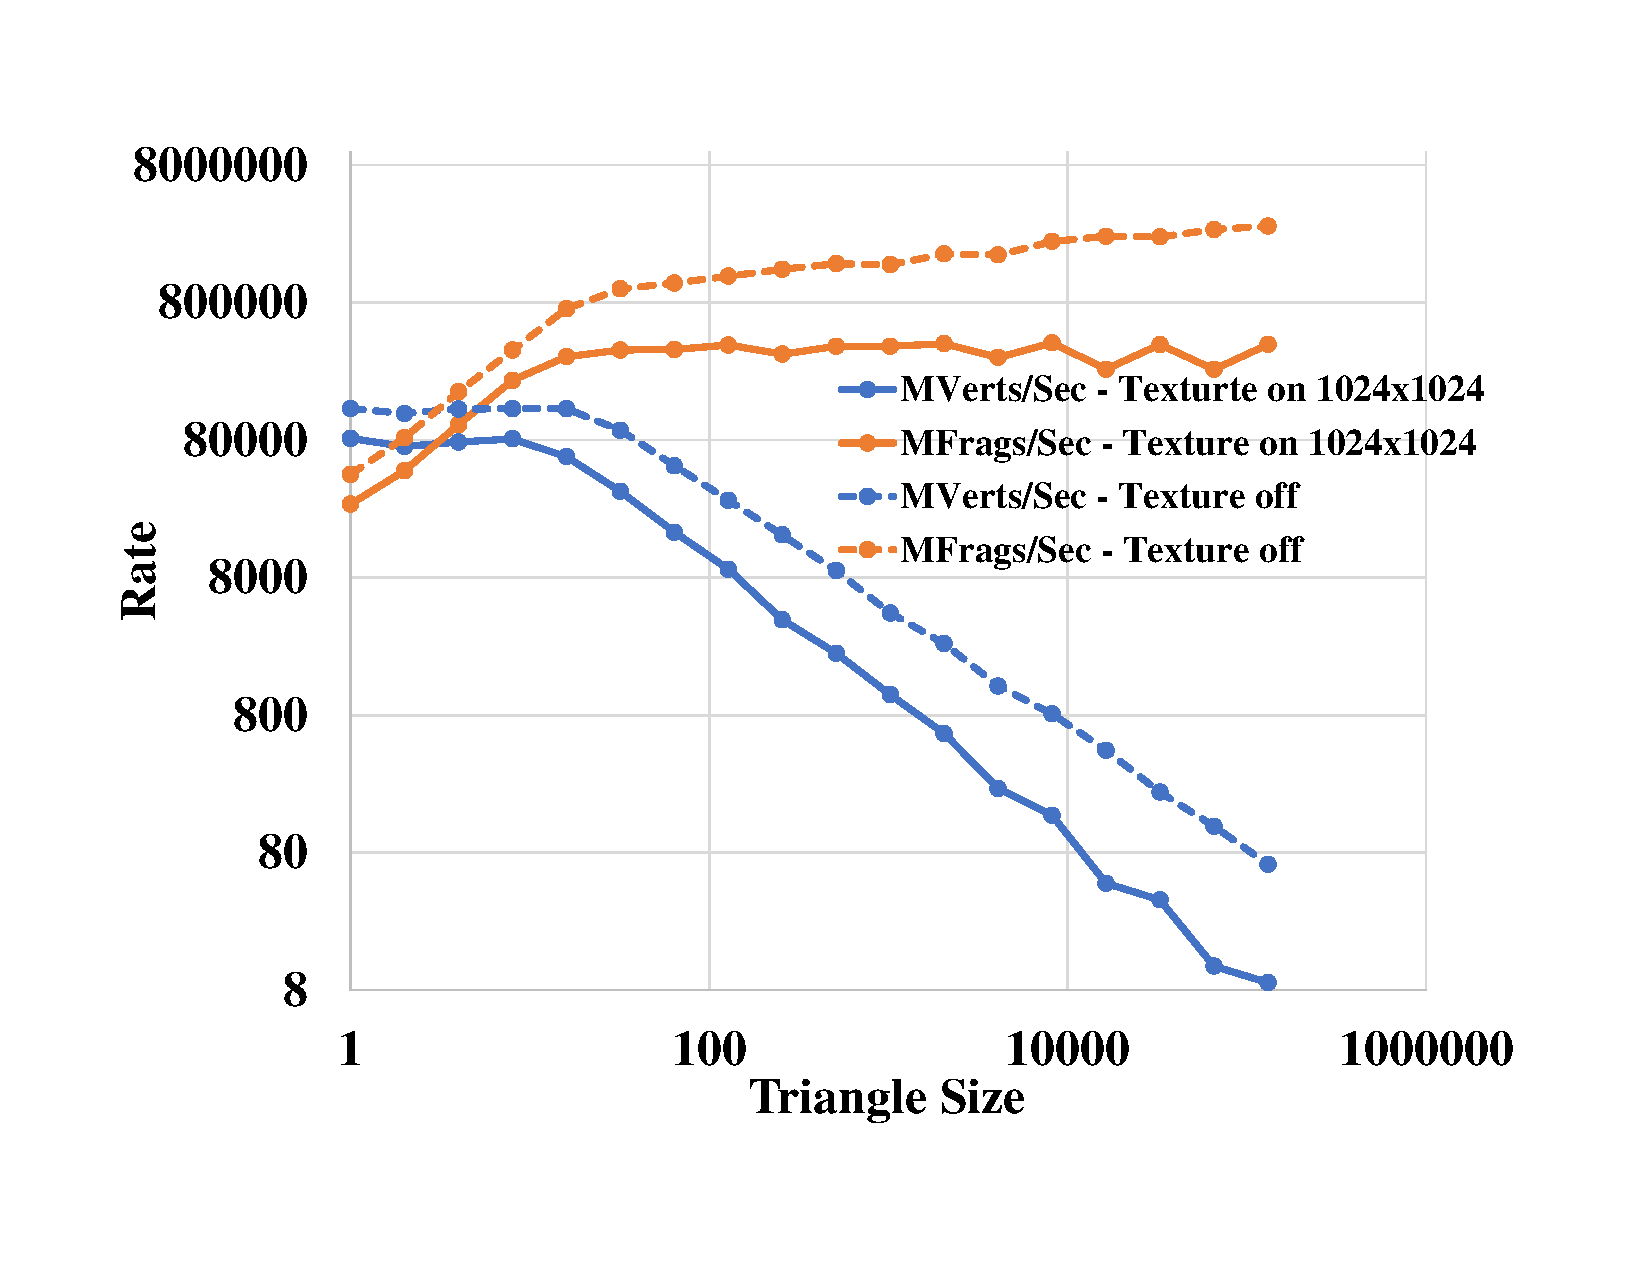
\includegraphics[width=0.49\linewidth]{fig/fill_geo_tx.pdf}}   
 \subfloat[Lit, Textured Triangles]
   {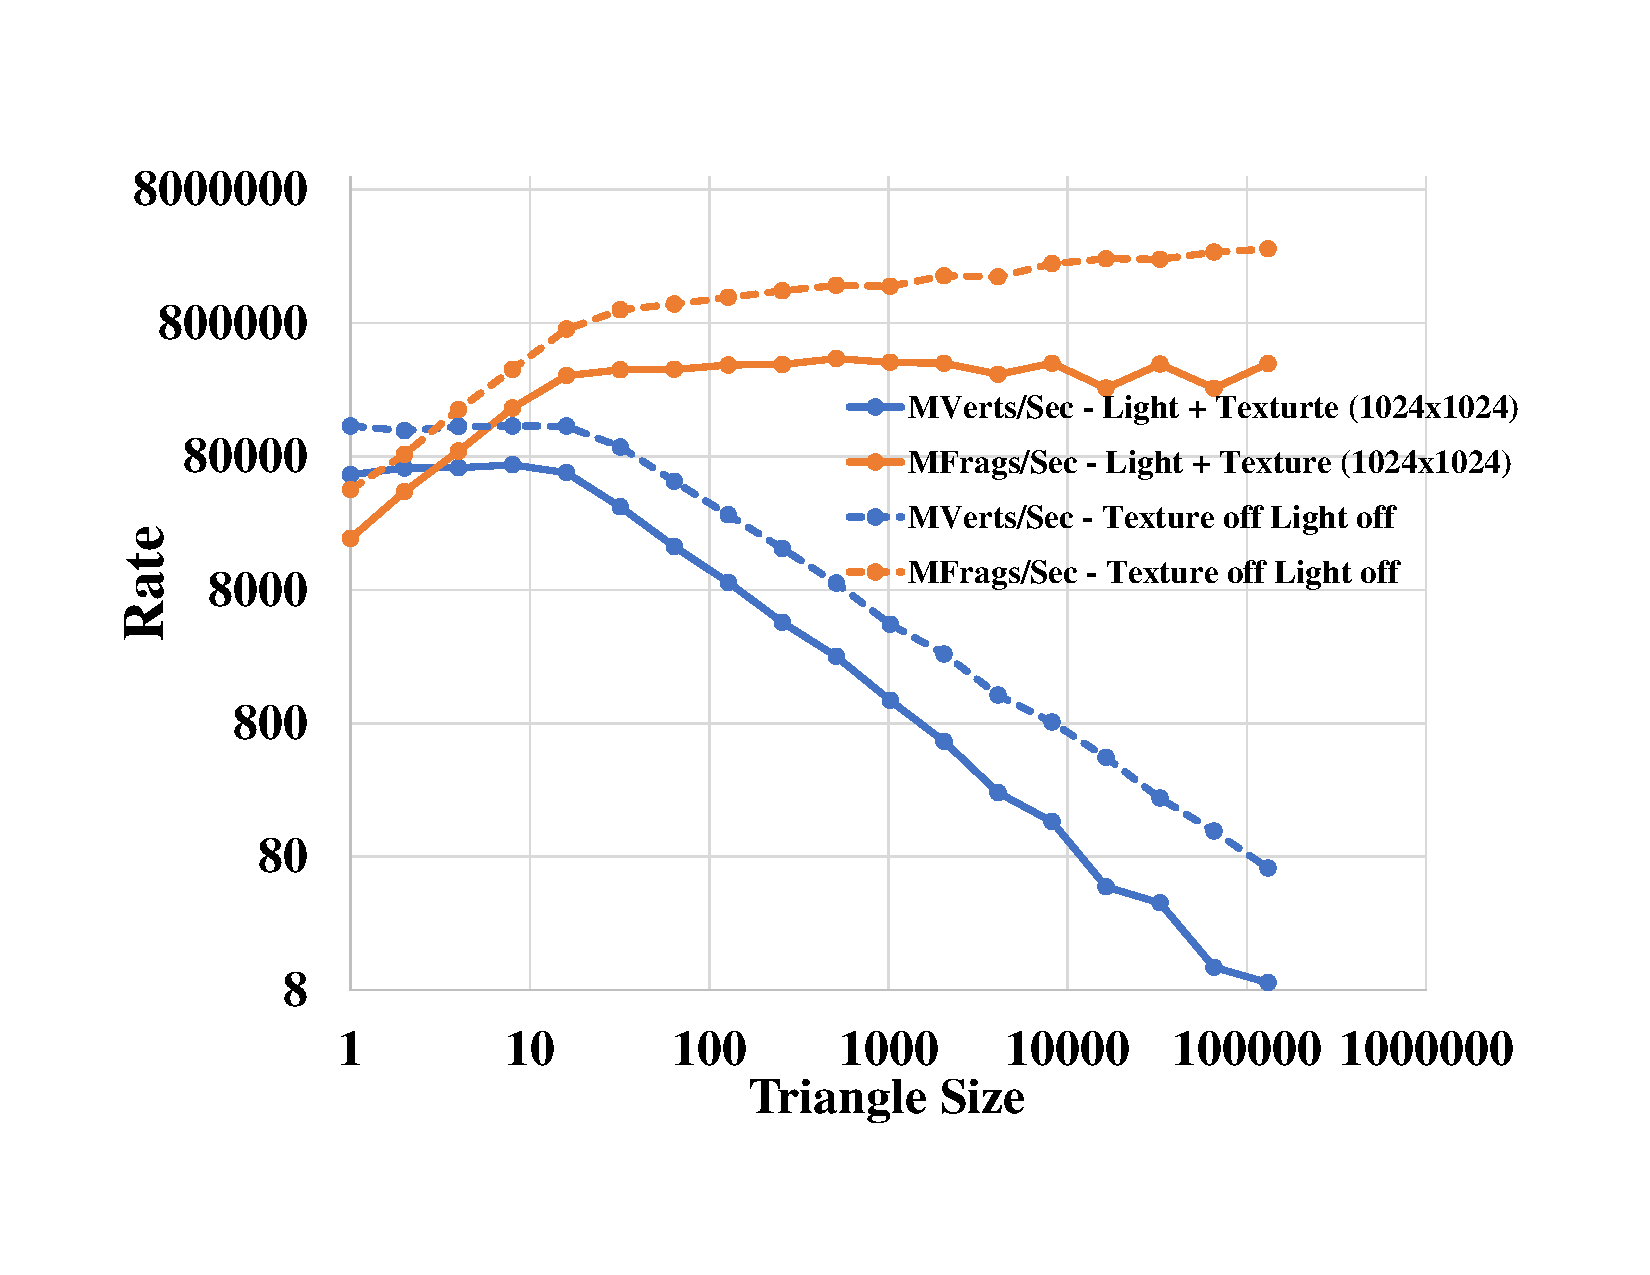
\includegraphics[width=0.49\linewidth]{fig/fill_geo_lit_tx.pdf}}
  \caption{Performance of the textured triangle Vs. the default (untextured) triangles in \protect{\wes} (a) and lit, textured triangles Vs. the default (unlit, untextured) triangles (b) in millions of vertices per second and millions of fragments per second.}
   \label{fig:fill_geo2}
\end{figure} 

%=========================Textured Triangles ===================================%
\subsection{Geometry Rate Vs. Fill Rate on Textured Triangles:}\label{sec:tx}
Now we turn on testing the textured triangles. Following the same methodology as in Section \ref{sec:lit}, we add textures of size $2^{7}\times2^{7}$ to the triangles and vary the triangle size and record the fill and geometry rates. We tested first with texture of smaller size ($2^{3}\times2^{3}$), but the graph we got was identical to the untextured one, so we discarded. We assume that this happened due to minimal workload required with small texture size. 

Figure \ref{fig:fill_geo2}(a), compare the fill and geometry rate for textured and untextured triangles. The crossover point has shifted to be between triangle of size $2^{12}$ and $2^{13}$ pixels. The graph also shows a decline in the performance in the textured triangles for both the geometry and fill rate. For the geometry stage, the decline in the number of vertices processed per second is due to the necessary transformation done per vertex (applying the \emph{projector function}\cite{akenine2008real}). The graph in Figure \ref{fig:fill_geo1}(b) and in Figure \ref{fig:fill_geo2}(a) suggest that per-vertex-operation for the lighting is similar to per-vertex-operation for texture which is indicated by the absolute value of geometry rate at a triangle size (for triangle size $\leq 2^{5}$ pixels). Additionally, the graph shows a divergence in the geometry rate between the textured and untextured curves. At first glance, this was surprising and we expected a similar behavior as in lit triangles (the curves overlap for large triangles). This stemmed from the fact that as the number of triangles decreased as the size increases, less number of vertices needed to be processed. However, we think that this divergence could be due to caching. Since we are using a relatively large texture ($2^{7}\times2^{7}$) and for a big triangles, it is required to fetch different parts of the texture image that may not be fetched all together into the cache (less spatial locality).

For rasterization, the fill rate decline since the texture operation is more expensive on fragments. During the rasterization, the \emph{corresponder function} (matrix transformation) is applied per fragment and texture value per fragment is interpolated \cite{akenine2008real}. Both could be the reason for the decline in the fill rate. We notice a similar divergence happens in fill rate. This is understandable since for large triangle more fragment are being processed per triangle (less parallelism can be extracted for big triangles).

%========================= Lit Texture Triangles====================================%
\subsection{Geometry Rate Vs. Fill Rate on Lit, Textured Triangles:}
Here we use lit, textured triangles and compare the same performance metrics with the unlit, untextured triangles. Figure \ref{fig:fill_geo2}(b) shows that the crossover point did not change from the texture triangle case (Section \ref{sec:tx}) which might indicate that the graphics card used is optimized for this value. For large triangles (size $\geq 2^{5}$) the lighting does not have real impact on both the geometry or the fill rates, then the decline in the performance is purely due to the texture processing. For smaller triangle size, both lighting and texturing contribute in the performance decrease.
%========================= Strip Vs. Disjoing Triangles====================================%
\subsection{Geometry Rate Vs. Fill Rate for Strips Vs. Disjoint Triangles:}
OpenGL offers to represent a set of triangle in form of a list allowing more efficient memory usage. The list (strip) offers substantial reduction in number of vertices needed to be processed. Instead of storing each triangle by its three vertices, strip stores a list of vertices such that each three vertices compose a triangle. Disjoint triangle store a triangle by its three vertices, thus almost all vertices are duplicated by the number of triangles a vertex is a member in. 

We use \protect{\wes} to measure the relative performance of the fill rate and geometry rate using these two types of triangle. The results is show in Figure \ref{fig:fill_geo3}(a). First we notice that the triangle rate of strip triangle is almost identical to the vertex rate. Meanwhile for disjoint triangle, the vertex rate is three time higher than the triangle rate (at certain triangle size). The reason behind that is the triangle strip length is equal to number of vertices plus two, thus we notice for very large triangle the two curves (triangle and vertex rate) diverge. 

An interesting observation is the vertex rate for triangle size $\geq 2^{4}$ for triangle strip is so close to this of disjoint triangle. This gives disjoint triangle higher performance in terms of vertex rate since the vertex rate is three time higher than the triangle rate. For smaller triangle size, strip triangle has higher triangle rate, but still vertex rate of disjoint triangle outperforms. This is because the triangle rate should be three times higher to start overcome the disjoint triangles. For fill rate, triangle strips outperforms the disjoint triangles. We assume that this is because both can feed the rasterization stage equally (similar triangle rate), but triangle strip exhibits better temporal and spatial locality which gives it an edge over disjoint triangle. 


%========================= Disjoing Vs. ID Disjoing Triangles==============================%
\subsection{Geometry Rate Vs. Fill Rate for Indexed Disjoint Vs. Disjoint Triangles:}
Here we try to evaluate the performance with two different type of triangles; disjoint and indexed disjoint triangles. With disjoint triangles, each triangle is specified by three vertices without reusing these vertices for a neighbor triangle. Indexed disjoint triangles reuse the vertices such that one vertex is shared among many triangles and thus no duplication is necessary. We will see later that the average number of triangles shared per vertex is approximately six triangles. 

For indexed disjoint triangle, the total number of vertices is reduced by factor of three. Thus, we expect the geometry rate to be higher for the case of indexed disjoint triangles when compared with disjoint triangles. But actually this not the case as shown in Figure \ref{fig:fill_geo3}(b) where the disjoint triangles geometry rate outperforms the indexed variant. If we, instead, look at the triangle rate (MTris/Sex), we will find that the triangle rate is identical for triangle of size $\geq2^{5}$. This means if the geometry stage is processing $X$ triangles, then for the disjoint triangles case, $3\times X$ vertex should be processed. But for the indexed disjoint case, less number of vertices will be processed. For triangle size $\geq2^{5}$, by dividing the the geometry rate for the disjoint triangle by the geometry rate for indexed disjoint triangles and taking the normalized average, the result would be the number of triangles shared per vertex in the indexed disjoint triangles. Rounding the result, we found that it is 6 triangles per vertex. In conclusion, this indicates that the graphic card must been optimized to handle both cases efficiently by fixing the number of triangles being processed regardless to the vertex rate (which sounds a complicated task to achieve!)

For fragment rate, since the geometry stage in both cases is able to send the same workload (in terms of triangle rate) for triangle of size $\geq 2^{5}$, we the fragment is almost identical for both cases with few wiggles that could be due to caching behavior in the disjoint case. Additionally, when the triangle rate increases for index disjoint triangles (triangle size $2^{1}-2^{5}$), we notice an equivalent improvement in fragment rate. The reason behind that is for such small triangles, the process is limited by geometry stage. If the geometry rate improves (able to send more work to rasterizer), then fill rate will improve too. 

We conclude from this comparison that we should also investigate the triangle rate, along with the vertex rate and fill rate in order to fully characterize and understand the graphic card behavior.
\begin{figure}[!tbh]
 \centering  
 \subfloat[Strips Vs. Disjoint]
   {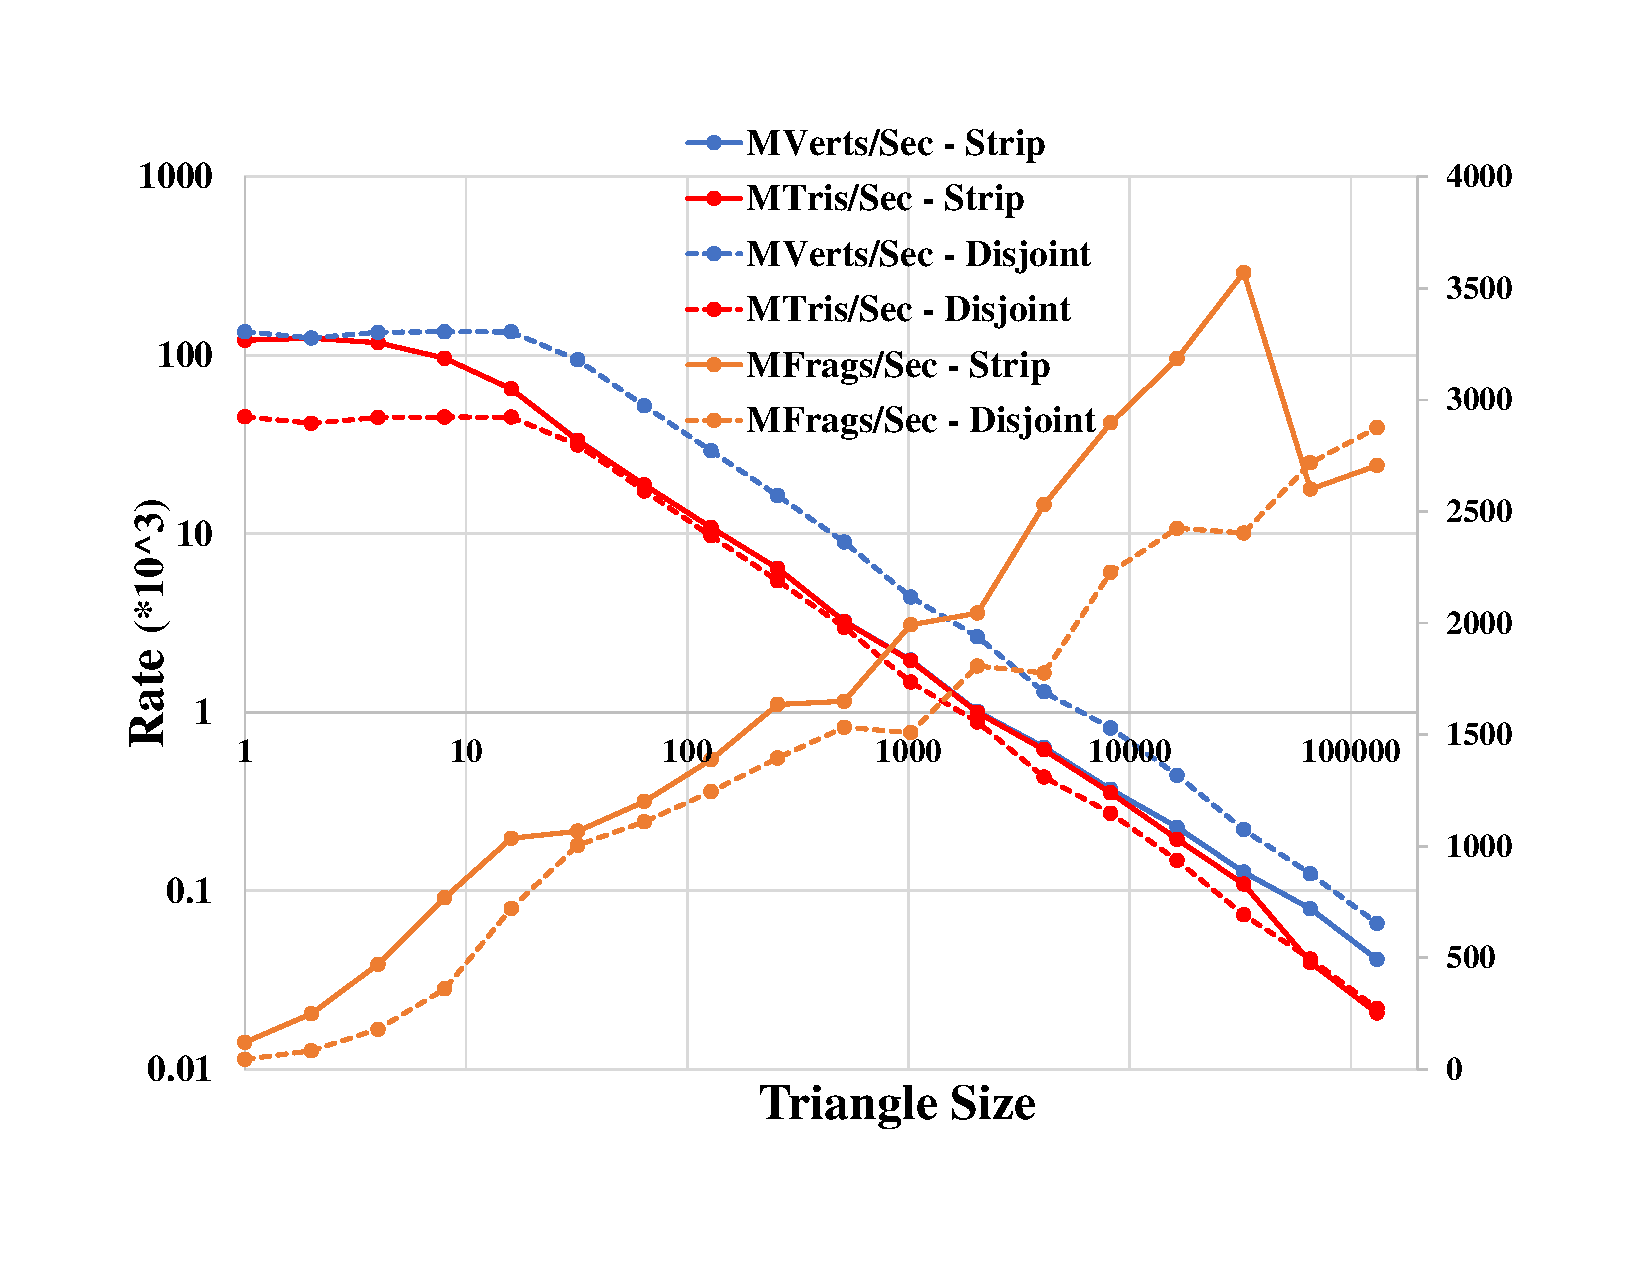
\includegraphics[width=0.49\linewidth]{fig/fill_geo_disj_tstrip.pdf}}
 \subfloat[Indexed Disjoint Vs. Disjoint]
    {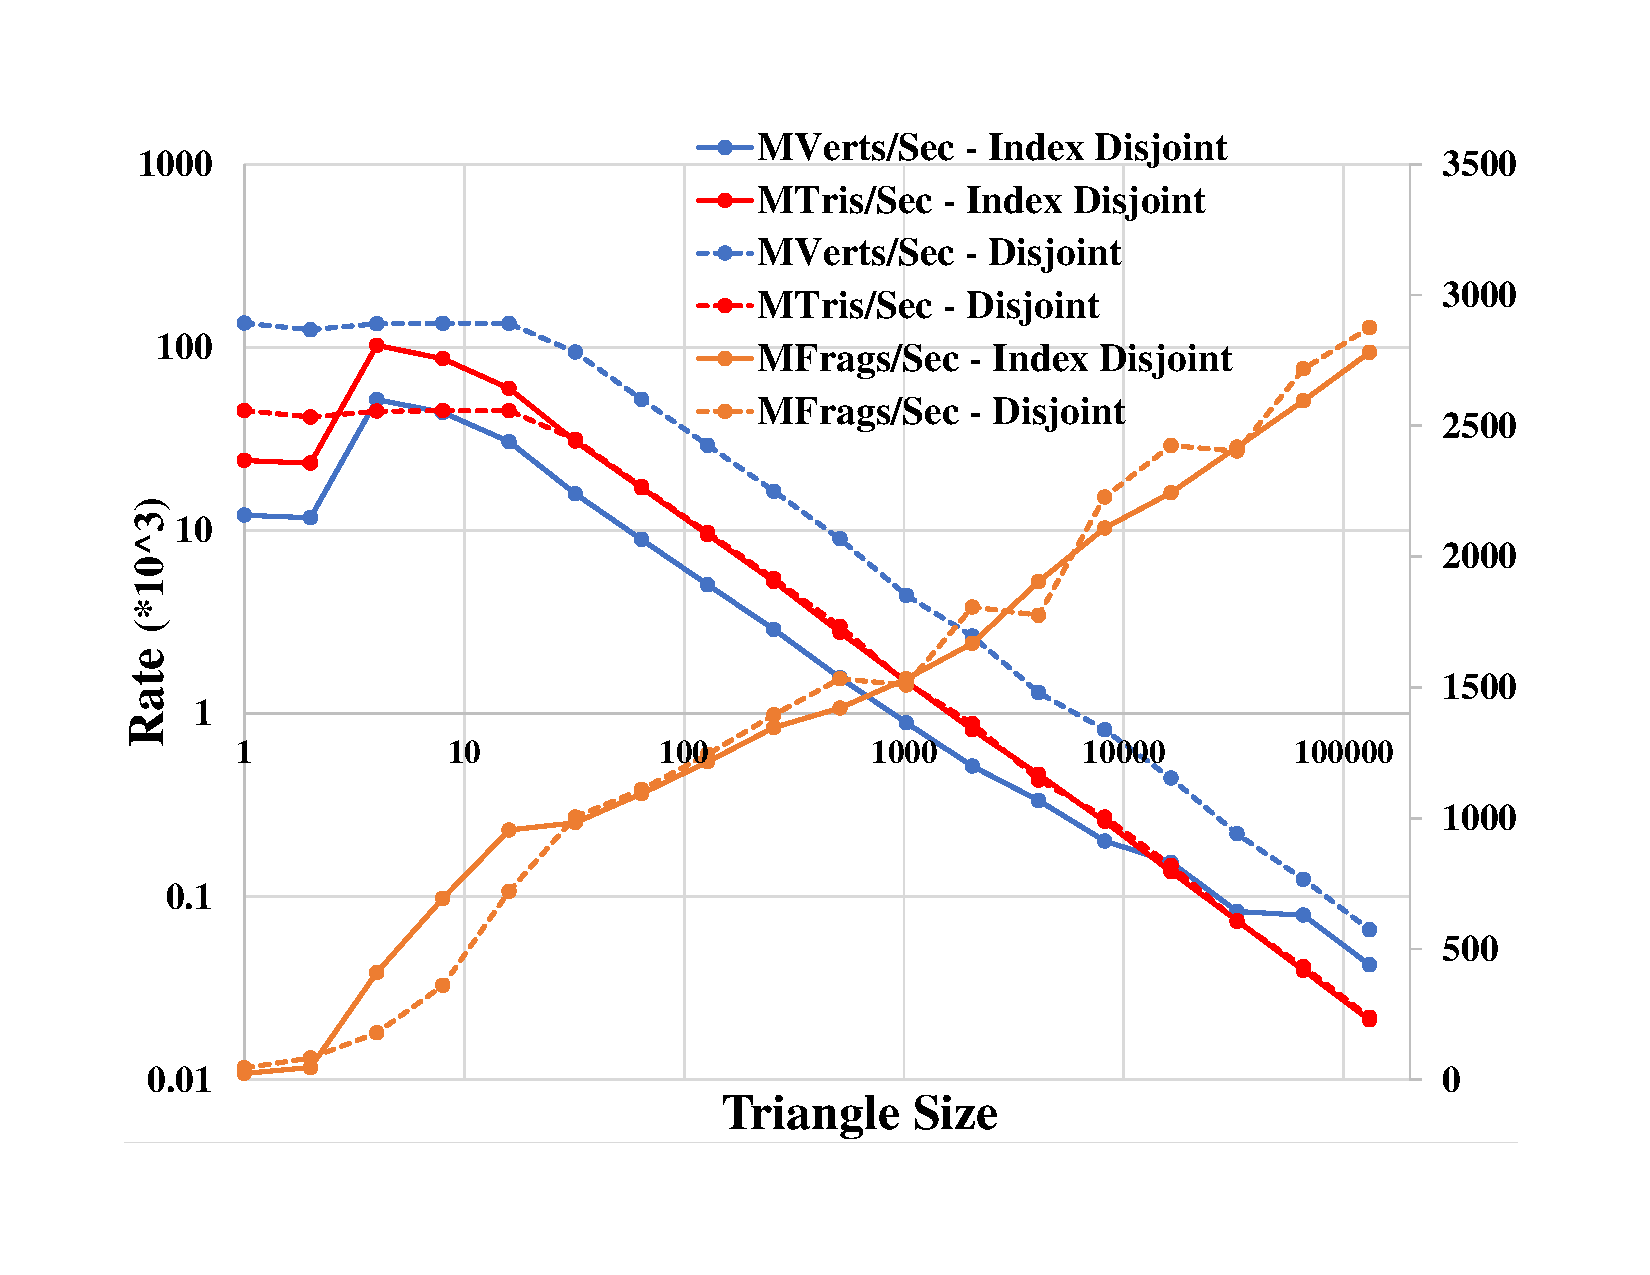
\includegraphics[width=0.49\linewidth]{fig/fill_geo_disj_IDdisj.pdf}}    
  \caption{Performance of the strips triangles Vs. disjoint triangles (a) and indexed disjoint triangles Vs. disjoint triangles (b) in millions of vertices per second, millions of triangle per second, and millions of fragments per second. }
   \label{fig:fill_geo3}
\end{figure} 


%========================= Batch Size TStrip Triangles====================================%
\subsection{Geometry Rate Vs. Fill Rate for Varying Batch Size:}

%========================= Batch Size TStrip Triangles====================================%
\subsection{Geometry Rate Vs. Fill Rate for Varying Texture Size:}
The final experiment was conduced to characterize the texture size and understand how it affects the performance. We used \protect{\wes} to vary the size of the texture image from $4\times4$ texels to $64\times64$ texels and recorded the vertex, fill, and triangles rates for two different triangle size as shown in Figure \ref{fig:fill_geo5}. We notice degradation in both the vertex rate and fill rate as the size of texture size increases. The decline in vertex rate (and triangle rate) is less dramatic than fill rate. For both vertex and fill rate, we assume the performance declines due to caching. For smaller texture size, the texture image can fit in the texture cache memory. Thus, the performance is limited by the operation itself. For larger texture size, the texture memory bandwidth is the bottleneck due to the repeated look-ups since the texture image could not be resident in the cache all the time. For fill rate, we would expect that the fill rate would remain constant for a range of texture size after which the fill rate would fall. Such a value would give an indication for the texture memory cache. But it looks like the cache is optimized (e.g. pre-fetching) such that the degradation in performance as the texture size increases is less dramatic. 

\begin{figure}[!tbh]
 \centering  
 \subfloat[Triangle area = $2^{7}$ pixels]
   {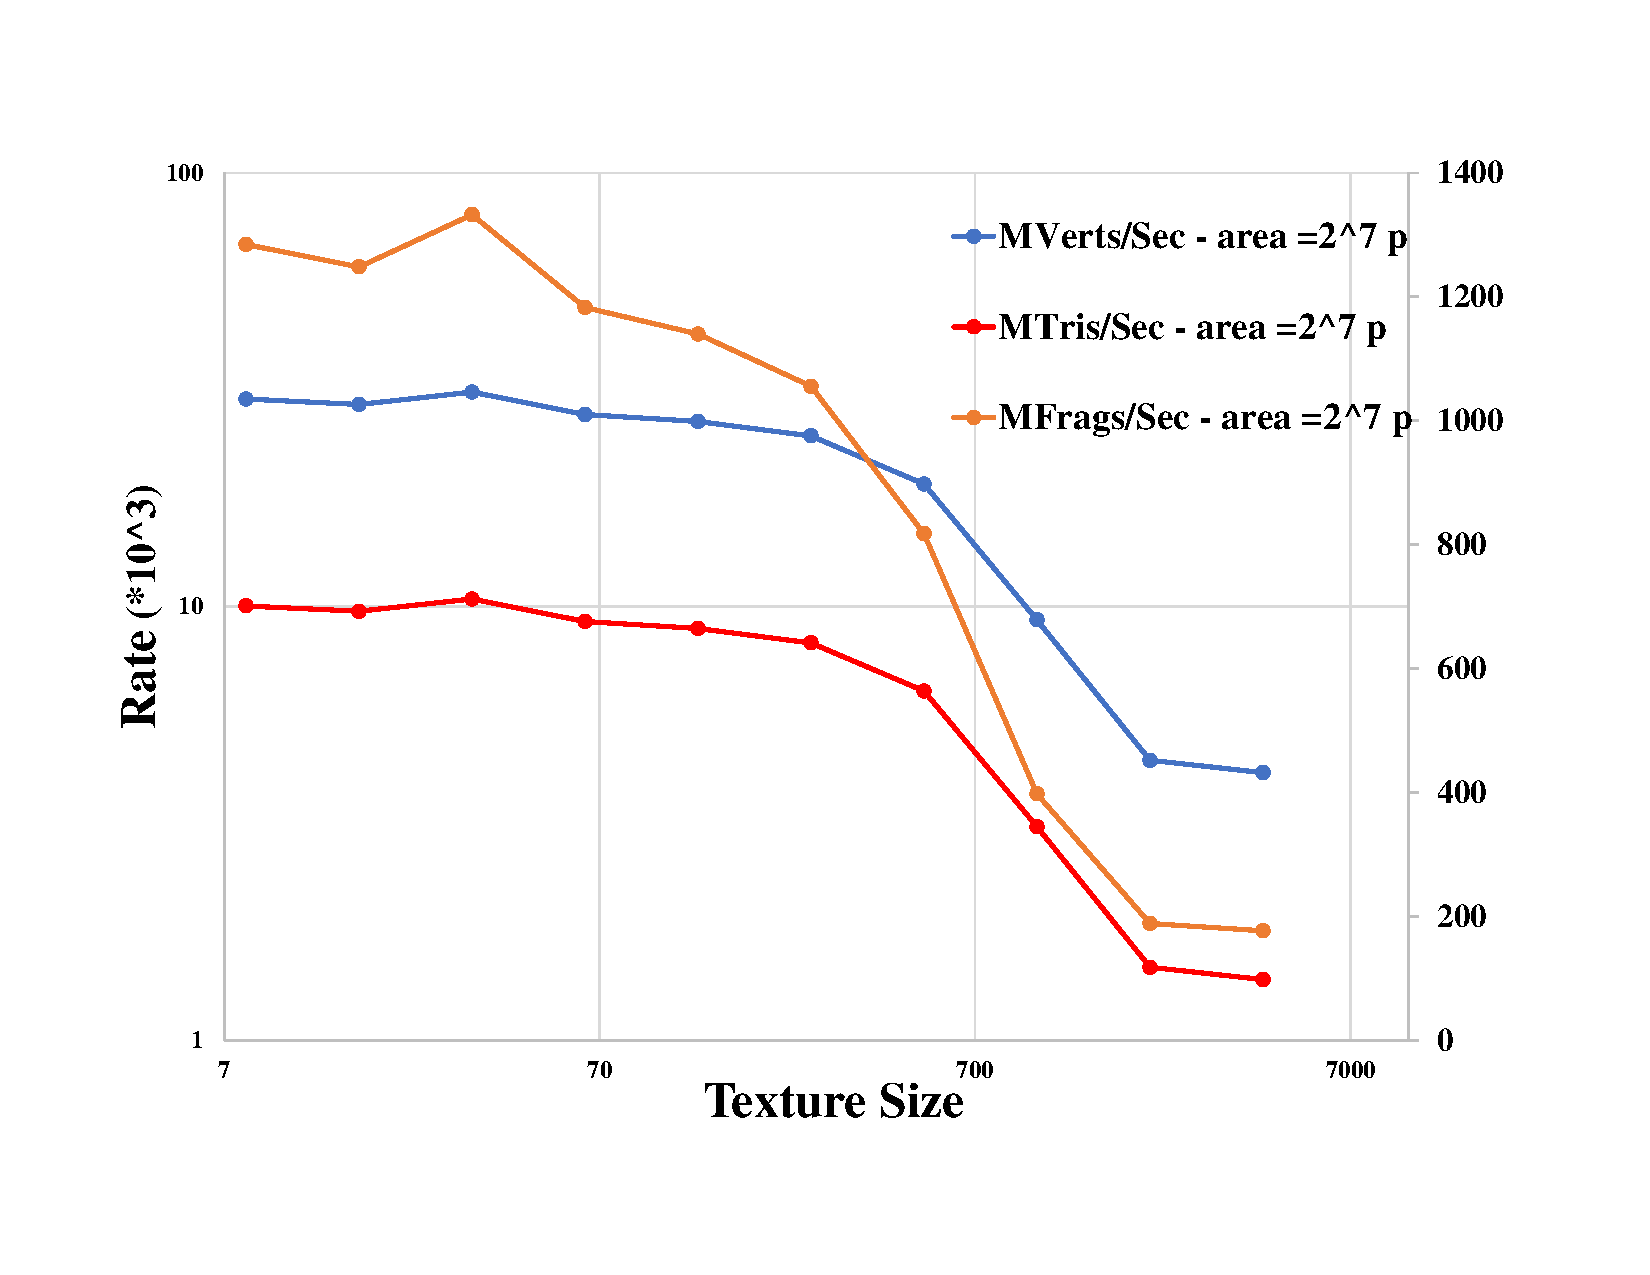
\includegraphics[width=0.49\linewidth]{fig/texture2_7.pdf}}
 \subfloat[Triangle area = $2^{14}$ pixels]
    {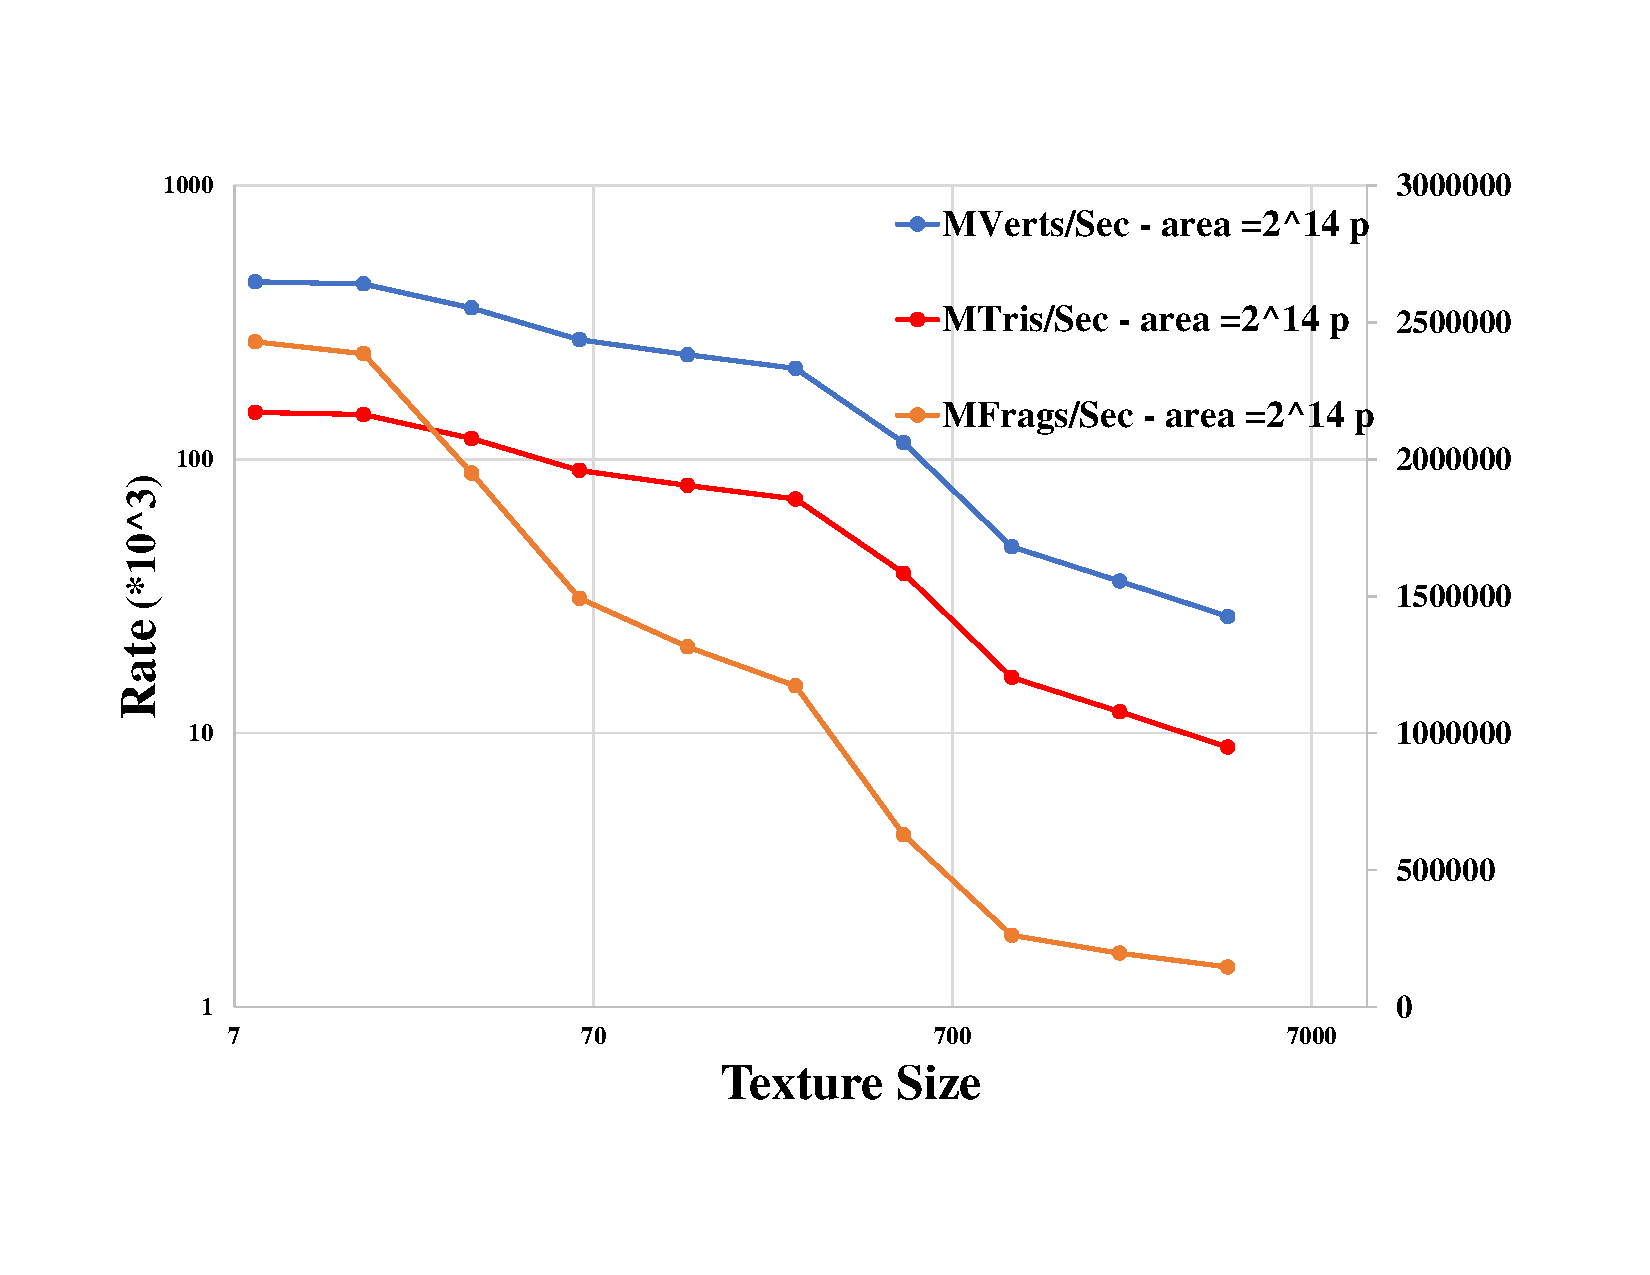
\includegraphics[width=0.49\linewidth]{fig/texture2_14.pdf}}    
  \caption{Performance of varying the texture size while fixing the triangle are to $2^{7}$ pixels (a) and $2^{14}$ pixels (b) in millions of vertices per second, millions of triangle per second, and millions of fragments per second. }
   \label{fig:fill_geo5}
\end{figure} 


\newpage

\section{Part B}
%=========================Intro====================================%
So far the characterization of the graphics card performance was in terms of the speed of operations. Now we turn to characterize the quality, specifically the arithmetic precision. This is considered a crucial since the speed render irrelevant if the results are not accurate. Even under the IEEE-754 Standards, identical operations could produce different results when operated on two different machines (e.g. floating point addition is not associative). 

In this section, we start by quantifying the error of the basic arithmetic operations offered by OpenGL. We compare GPU's results with the CPU to measure the error. We also try to discover a precision-related undocumented features; how rounding is implemented in our graphic card. 

%=========================Arithmetic Opt====================================%
\subsection{Arithmetic Operations Accuracy:}
Here we test a range of basic arithmetic operation offered by OpenGL and GLSL. Taking the CPU results as our datum, the absolute relative error between the GPU's results and CPU's results represents the GPU errors. The rationale behind this method is that both CPU and GPU are compliant with IEEE-754 Standard. %We will revisit this idea in Section \ref{sec:dot}, where we see careful implementation could make the graphic card more accurate. 

%=========================Dot Product====================================%
%\subsection{Dot Product}\label{sec:dot}
%Here we performance dot product between two float vectors and measure the error between the 
%\cite{whitehead2011precision}

%=========================Rounding====================================%
\subsection{Rounding}
The purpose of this test is to first verify that our GPU is IEEE-754 compliant and second to identify the rounding algorithm implemented. For this test, we borrowed the fragment shader used in Russell's article \cite{stuart2013mobile} shown in Figure \ref{fig:shader1}. In Russell's article, the shader was used to benchmark the accuracy of GPU floating point across different mobile GPUs. 

The shader simply fills the screen with 26 bars. Given infinite precision, each bar should vary linearly from white (left) to black (right) as a function of $X$ coordinate of the pixel. The shader is written such that with each level/bar, one bit of the fraction is thrown away. For each level $L$, we add $2^{L}$ to the computed gray value ($X$ coordinate of the pixel) and take the fraction of the result. The added integer ($2^{L}$) does not affect the value of the gray scale, but only its precision. For example, for the first bar, we add  $2^{L}=(1)_{ten}=(1)_{two}$ which is represented by one bit. Thus, when added to $fract(x)$ and taking the $fract()$ of the result, we only loss one bit of the $x$ precision. For the next level, we add $2^{L}=(4)_{ten}=(10)_{two}$, which is represented by two bits and thus two bits loss in $x$ precision. This goes up till we end up with zero precision in the fraction part and thus the image turns to black. Figure \ref{fig:prec} shows the result of running the shader on our graphic card. We can see that even though we are trying to draw 26 bars, only 23 bars are shown and the rest are black. This verifies that the fraction part of float in our graphic card is represented by 23 bits which matches exactly what IEEE-754 requirements. 

\begin{figure}[t!]
\centering
\begin{minipage}[t]{\textwidth}
\centering
\begin{lstlisting}[label=list:ExampleShader,
escapechar=|,
caption={
  Fragment Shader.
}]
void main(void) {
  float y = (gl_FragCoord.y / 600) * 26.0
  float x = (1.0 -(gl_FragCoord.x / 800))
  float yp = pow(2.0, floor(y))
  float fade = fract(yp + fract(x))
  if (fract(y) < 0.9)
     gl_FragColor = vec4(vec3(fade), 1.0)
  else
     gl_FragColor = vec4(0.0)
}
|
\end{lstlisting}
\end{minipage}

\caption{The fragment shader implementation for verify the floating-point representation compliance with IEEE-754 standards}
\label{fig:shader1}
\end{figure}


\begin{figure}[t!]
 \centering   
 \subfloat[Precision Shader]
    {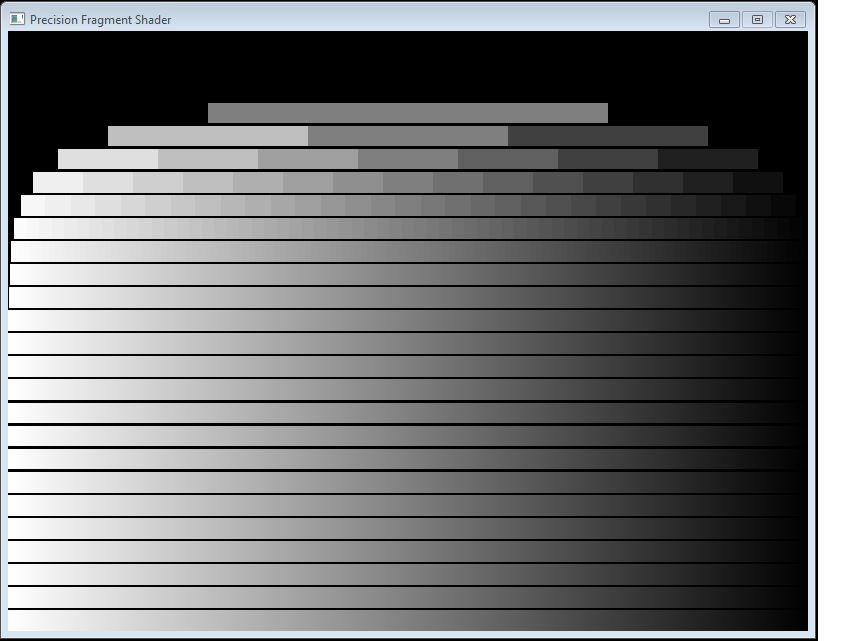
\includegraphics[width=0.49\linewidth]{fig/shader.JPG}} 
 \subfloat[blah]
   {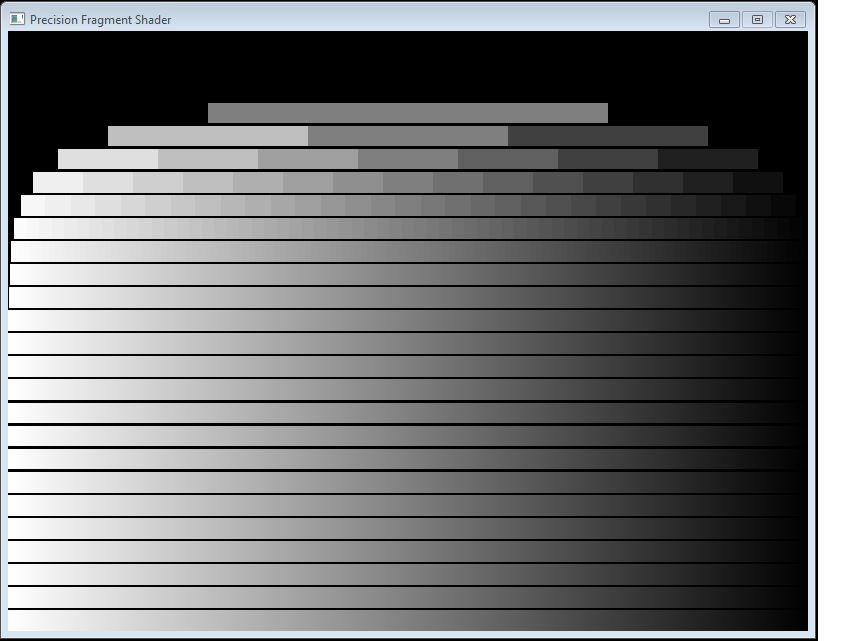
\includegraphics[width=0.49\linewidth]{fig/shader.JPG}}   
  \caption{Results of applying shader in Figure \ref{fig:shader1}  on our graphic card.}
   \label{fig:prec}
\end{figure} 







\newpage

\section*{Appendix}
%=======================some insights over wesBench implementatio==============================%

\ahmed{TODO: talk about the OpenGL calls in the code i.e., "Why do we use glDrawXXX calls rather than glBegin, glVertex, glEnd calls to draw geometry?", "What is wesBench actually drawing?" and "How does wesBench make sure that all geometry that it draws will pass through the entire pipeline?"  }

We answer here few questions concerning the implementation of \protect{\wes}. This can be considered as the lessons we have learned after dealing with \protect{\wes} code.

Using glDrawArray or glDrawElement is faster and more efficient than using glBegin, glVertex, glEnd. Basically, using glDrawXXX allows us to use the notion of Vertex Buffer Object (VBO) which treats a set of vertices as one group as opposed to the direct mode of processing one vertex at a time. Using VBO shows improved performance when using large batches of vertices. Also using the VBO comes in handy with programmable shading. We can write a shader program to specify how our pipeline should manipulate the vertices’ attributes and that will apply to all elements in the VBO automatically. The old school, now deprecated, glBegin/glEnd approach relays on explicitly describing the attributes of each vertex. In \protect{\wes}, they use VBOs to send data to the GPU as a single array contains position data followed by color data, etc. This allows making one function call to draw the arrays rather than several calls.
\protect{\wes} is actually drawing its geometry by constructing a $M\times M$ mesh of points that are positioned to fill one quarter of the screen resolution. The spacing between vertices in that mesh is specified by user inputted area of the triangles. This mesh is converted in the pipeline to fragments. \protect{\wes} makes sure that all the fragments should remain visible while rotating the mesh about the center of the screen for user-specified time duration.



%=========================Bib====================================%
\bibliography{mybib}
\bibliographystyle{IEEEtran}

\end{document}
